%!TEX root = forallxsyr.tex
\thispagestyle{empty}


    \begin{tikzpicture}[remember picture, overlay]%
      \node [xshift=10.5cm,yshift=6.3cm] at (current page.south west) {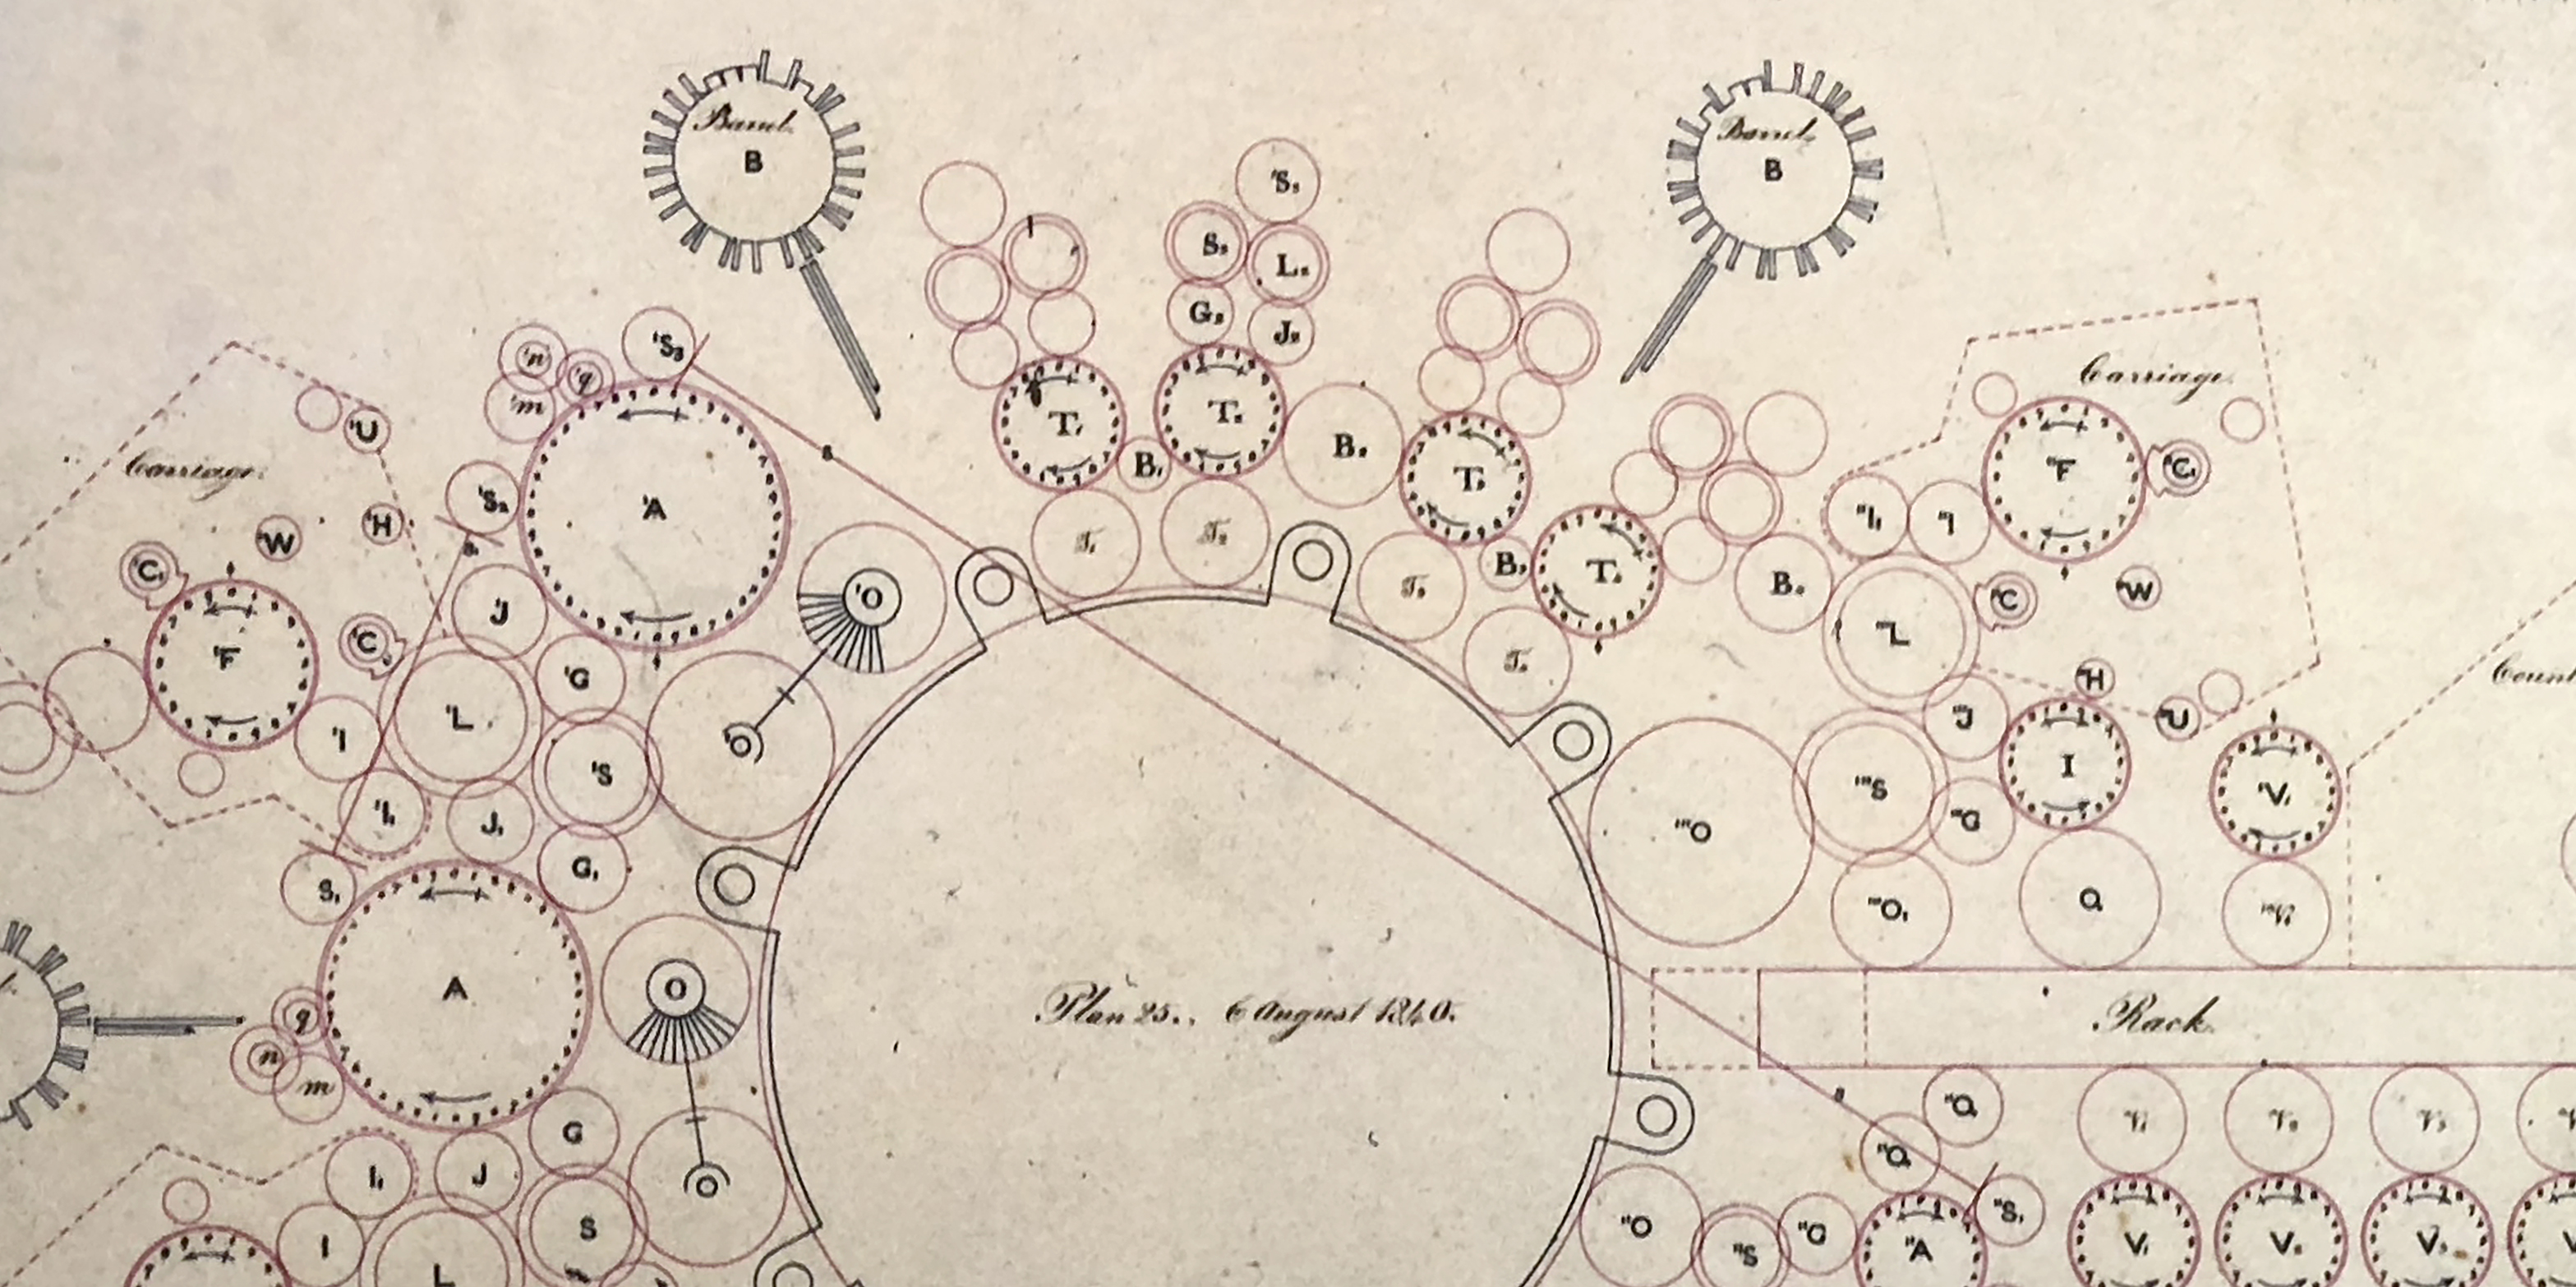
\includegraphics[scale=0.95]{cover-image.jpg}};%
    \end{tikzpicture}
    
\vspace{20pt}
    
\begin{center}
\fontsize{36pt}{36pt}\selectfont
  \textbf{forallx@syr}

\fontsize{24pt}{24pt}\selectfont
\vspace{1em}
\textit{An Introduction to\\ Formal Logic}


\vspace{40pt}

\fontsize{16pt}{18pt}\selectfont By P.~D. Magnus, Tim Button, and Michael Rieppel\\

\vspace{85pt}

\fontsize{20pt}{20pt}\selectfont
Fall 2021 Edition
\end{center}

\newpage


\noindent \small \copyright \ P.~D. Magnus, Tim Button, and Michael Rieppel, 2005-2021

\vspace{1ex}

\noindent This book is based on \href{http://www.homepages.ucl.ac.uk/~uctytbu/forallxcam.pdf}{\emph{forall x: Cambridge}}, by  \href{http://www.homepages.ucl.ac.uk/~uctytbu}{Tim Button}
(UCL), used under a \href{https://creativecommons.org/licenses/by/4.0/}{CC BY 4.0} license.  Button's book is in turn based on the original \href{https://www.fecundity.com/logic/}{\emph{forall x}}, by
\href{https://www.fecundity.com/job/}{P.D.\ Magnus} (SUNY Albany), used under a \href{https://creativecommons.org/licenses/by/4.0/}{CC BY 4.0} license.

\vspace{1ex}

\noindent The present text, \emph{forallx@syr}, was revised and expanded by \href{https://mrieppel.net/}{Michael Rieppel} (Syracuse University).  This work is licensed under a \href{https://creativecommons.org/licenses/by-sa/4.0/}{CC BY-SA 4.0} (Creative Commons Attribution-ShareAlike 4.0) license.  You are free to copy and redistribute the material in any medium or format, and  remix, transform, and build upon the material for any purpose, even commercially, under the following terms:
\begin{itemize}
\item Attribution -- You must give appropriate credit, provide a link to the license, and indicate if changes were made. You may do so in any reasonable manner, but not in any way that suggests the licensor endorses you or your use.

\item ShareAlike -- If you remix, transform, or build upon the material, you must distribute your contributions under the same license as the original.

\item No additional restrictions -- You may not apply legal terms or technological measures that legally restrict others from doing anything the license permits.
\end{itemize}

\vspace{1ex}
\noindent Cover Image: plan for Babbage's Analytical Engine (1840). Available at \href{https://commons.wikimedia.org/wiki/File:Babbage_Analytical_Engine_Plan_1840_CHM.agr.jpg}{Wikimedia Commons}.

\vspace{1ex}

\noindent The \LaTeX{} source for this book is available on GitHub at \href{https://github.com/mrieppel}{https://github.com/mrieppel}. 

\vspace{1ex}

\noindent The present version was released on \today.

\vspace{1ex}
\noindent Thanks to Yasmeen Hembree, Scott Looney, Thiago de Melo, Ian York, and Yulun Zeng for spotting typos, errors, or omissions in earlier versions.

\newpage
\normalsize
\chapter*{Preface}

I first learned formal logic from Michael Byrd at UW-Madison, using Lemmon's  \emph{Beginning Logic}, and first taught logic in 2008 as a teaching assistant for Branden Fitelson at UC Berkeley, using Forbes' \emph{Modern Logic}.  When I started to develop my own logic course, I continued to use Forbes' book, which I liked for its thorough treatment of the three central components of an introductory logic class: symbolization, semantics, and natural deduction.  

However, over time I became dissatisfied with \emph{Modern Logic} for two reasons.  First, the Lemmon-style notation that it uses for natural deduction is much less accessible to beginners than the Fitch-style notation found in other texts.  And second, Oxford University Press started printing fewer copies of the book, making it rather expensive --- more expensive, at any rate, than I thought an introductory logic text should be.  By the time I began teaching at Syracuse in 2015, I therefore started listing Forbes' book only as a recommended text, and relied heavily on the detailed lecture notes I had put together over the years.

But in the longer term, I faced a choice: either select a new textbook, or transform my own notes into a book.  The open-source nature of Tim Button's \emph{forall x: Cambridge} offered me way to do both: I could take his already excellent text (which \emph{inter alia} included a Fitch-style deduction system) and supplement it with material of my own.  And so I've come to make my own addition to the ``groaning shelves'' of logic textbooks, to borrow Forbes' description --- though with electronic distribution, the groan has thankfully become more metaphorical. The main additions I've made to \emph{forall x: Cambridge} are the following:
\begin{itemize}
\item I've changed the first chapter by e.g. elucidating the modal notion of validity using possible worlds, and emphasizing logic's focus on formal validity a bit more.
\item I've added more on the semantics of truth-functional and especially first-order logic, particularly as concerns the construction of countermodels.  
\item I've made some changes to the natural deduction rules in both parts.
\item I've reordered the presentation of various topics and revised the practice problems.
\end{itemize}
Besides the obvious debt the present text owes to the \emph{forall x} editions that P.D. Magnus and Tim Button have so generously made available,  and to Forbes' \emph{Modern Logic}, I also draw on ideas I've picked up from Barwise and Etchemendy's \emph{Language, Proof, and Logic}, Belnap's \emph{The Art of Logic}, Goldfarb's \emph{Deductive Logic}, \emph{forall x: Calgary Remix}, and lecture notes by Branden Fitelson,  Daniel Warren, and John MacFarlane.


